\section{Implementation}\label{sec:implementation}

The output of our algorithm can already be implemented in the commodity switches. In this section, we
describe the details of our implementation, starting by explaining how the commodity shared-buffer switch
maintains the queues and handles PFC.   

\subsection{Switch Model}\label{subsec:model}

\begin{figure}
	\hspace{-0.2in}
	\centering
		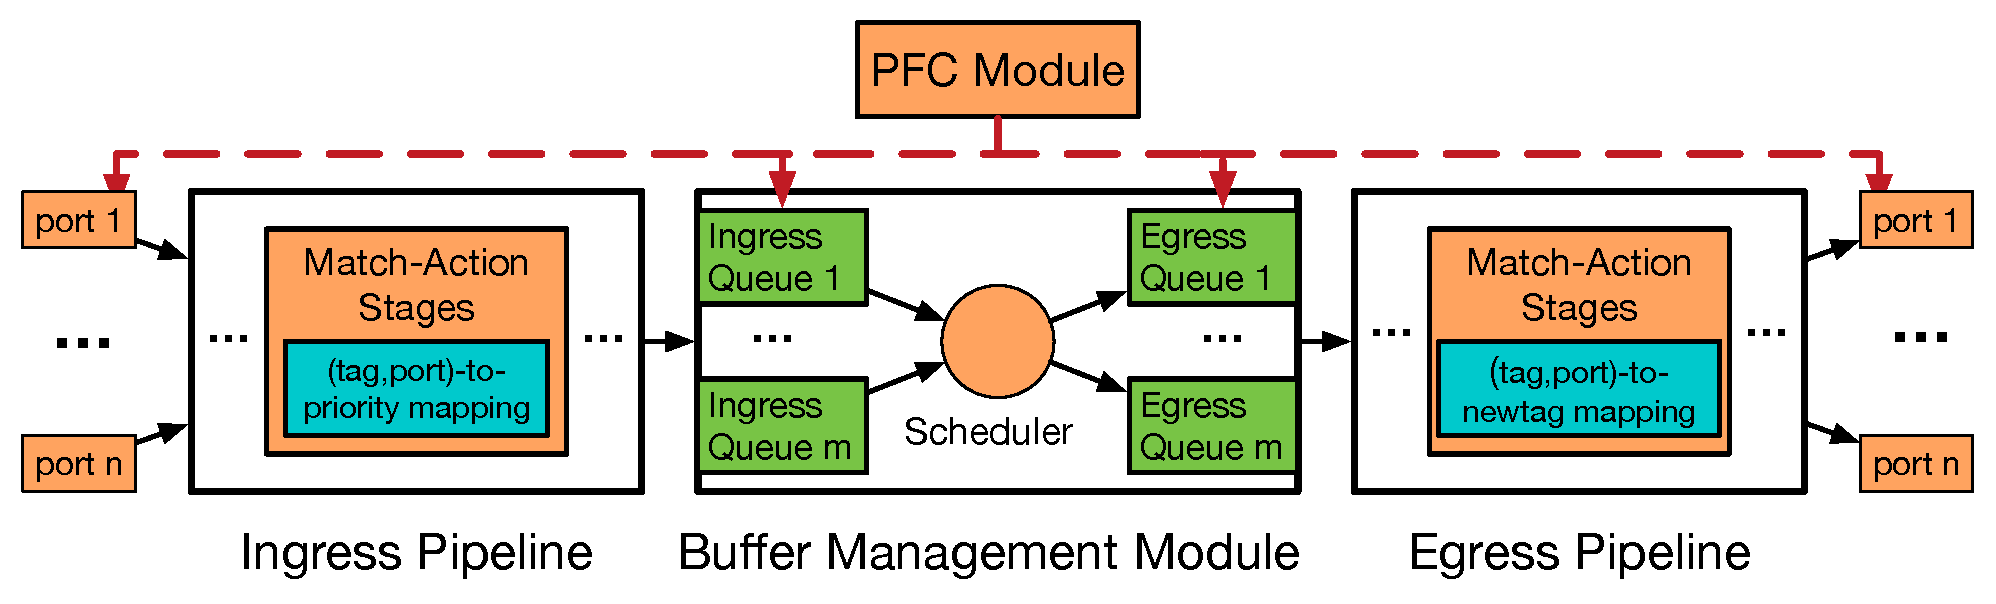
\includegraphics[width=0.5\textwidth] {figs/switch_model}
	\caption{Switch model.}\label{fig:switchmodel}

\end{figure}

In this part, we abstract the switch model on which we implement our algorithm output. 
Most commodity shared-buffer switches comply with this model. 
As shown in Fig.~\ref{fig:switchmodel}, our switch model consists of four modules: switch port, ingress pipeline, buffer management module and PFC module. The function of these modules are list as follows.

%Fig.~\ref{fig:switchmodel}(a) shows the architecture of the switch model, which consists of a switching fabric and N line cards. Line cards are mainly used to receive/send packets and make routing/forwarding decisions. Switching fabric is a module to transfer packet cells from the input line card to the output line card. 

\begin{itemize}
	\item \textbf{Switch port}: The module to receive and send packets.
	
	\item \textbf{Ingress pipeline}: The module to execute packet processing tasks before a packet enters switch buffer. These tasks include packet header parsing, L2/L3 lookup, ingress ACL processing, etc.  This module has multiple match-action stages to fulfill its tasks. Our \sysname{} is implemented here.
	
	\item \textbf{Buffer management module}: The module to manage switch buffer. This module has k ingress queues and k egress queues. The $i^{th}$ queue is corresponding to the $i^{th}$ priority class. Every ingress queue has n subqueues to buffer packets from n input ports. Similarly, every egress queue buffers packets destined for different output ports with n separate subqueues.
	
	Separate counters are used to track the queue length of each ingress subqueue and each egress subqueue. The ingress counter increases when a packet enters the ingress queue, and decreases when a queued packet leaves the switch buffer. Egress counter works similarly. 
	
	%Note that when a packet is forwarded to an egress queue from some ingress queue, the corresponding ingress counter will not decrease as this packet still remains in the switch buffer.
	
	\item \textbf{PFC engine}: The module to perform PFC function. If the switch receives a PFC PAUSE frame on priority class $i$ at some output port, this module will pause the $i^{th}$ subqueue of the corresponding egress queue. If the occupancy of some ingress subqueue exceeds the PFC threshold, this module will trigger the corresponding input port to send a PFC PAUSE frame to pause the upstream device on the corresponding priority. 

\end{itemize}


\subsection{\sysname{} Module}\label{subsec:acl}

\begin{figure}
	\hspace{-0.2in}
	\centering
	\includegraphics[width=0.5\textwidth] {figs/tagger}
	\caption{Tagger module.}\label{fig:tagger}
	
\end{figure}

 To build a tagging system for guaranteeing deadlock-free, we need to perform two operations at every hop in the network, i.e.,  {\em tag-based priority queueing} and {\em tag rewriting}. As shown in Figure~\ref{fig:tagger}, these two operations are implemented using a 3-step match-action pipelines. 
 
 In the first step, \sysname{} classifies packets into corresponding ingress queues based on the value of tags. In the second step, \sysname{} rewrites the value of tag based on (tag, inport, outport) information. The first two steps together enforce the tag hierarchical tree of the target tagging system. 
 
 
  \begin{figure}[t]
 	%\vspace{-0.1in}
 	\centering
 	
 	\subfloat[short for lof][Ingress priority = egress priority  $\rightarrow$ packet drop.] {
 		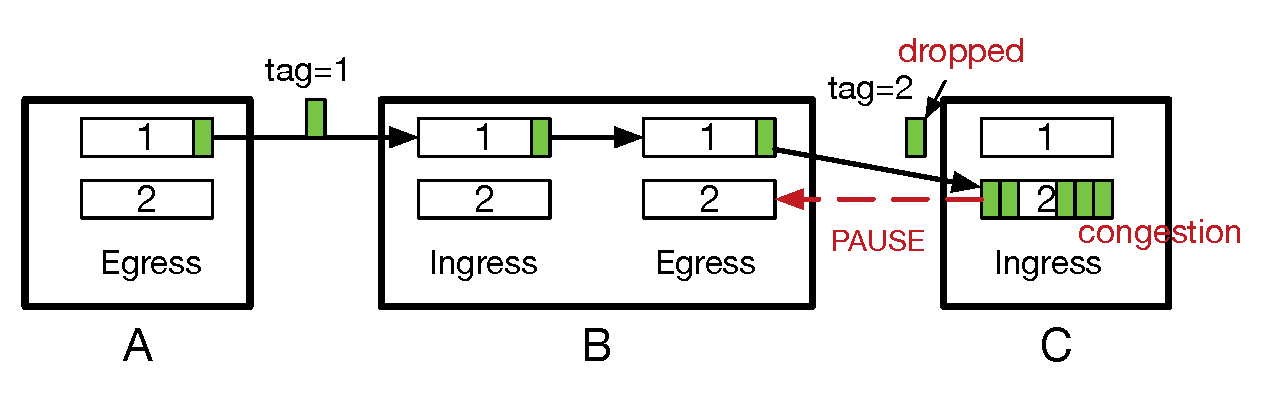
\includegraphics[width=0.43\textwidth] {figs/prioritydecoupling_1}
 	}
 	
 	\subfloat[short for lof][Ingress priority = 1, egress priority = 2 $\rightarrow$ no drop.]{
 		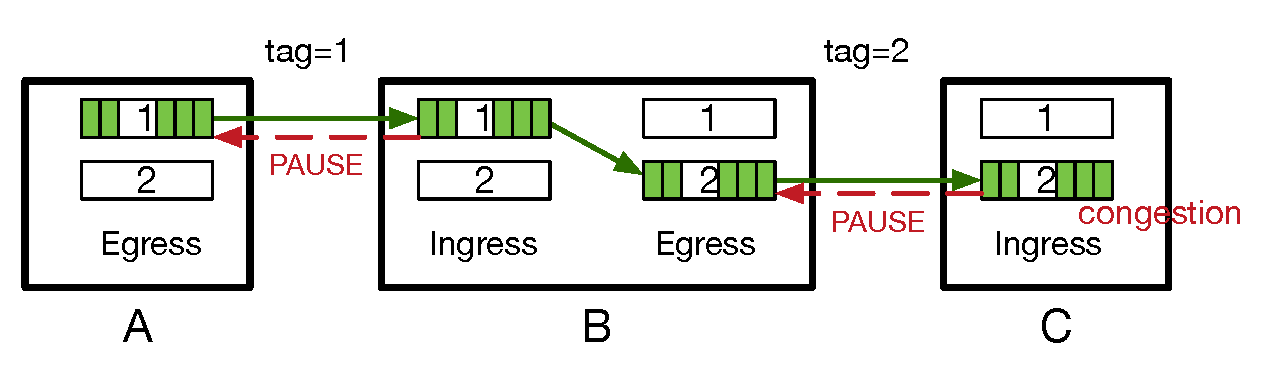
\includegraphics[width=0.43\textwidth] {figs/prioritydecoupling_2}
 	}
 	
 	
 	\caption{Decoupling ingress priority from egress priority at switch B is necessary for ensuring lossless priority transition.}\label{fig:prioritydecoupling}
 	
 \end{figure}
 
 Note that the tagged graph $G$ only defines the mapping between tags and ingress queues. The default switch configuration ensures a packet will be forwarded to the egress queue of the same priority class as its ingress queue. However, this default configuration may lead to packet loss when priority transition is performed. An example is shown in Figure~\ref{fig:prioritydecoupling}. 
 
 In this example, switch B is configured to do priority transition for packets received from switch A and destined for switch C.
 
 In Figure~\ref{fig:prioritydecoupling}(a), we consider the default switch configuration. Packets are forwarded to egress queue 1 at switch B. As we can see, this configuration leads to packet loss when ingress queue 2 of switch C becomes congested. This is because the PFC PAUSE from switch C to switch B cannot pause  egress queue 1 of switch B. 
 
 In Figure~\ref{fig:prioritydecoupling}(b), we let the ingress priority to be different from the egress priority at switch B. As we can see, packet loss is avoided when associating the egress queue with the new tag after doing tag rewriting.
 
 Based on the above observation, in the third step, \sysname{} classifies packets into corresponding egress queues based on the value of new tags. This ensures lossless priority transition.
 
 \textbf{\sysname{} Implementation on commodity switches.} We use DSCP filed in the IP header as the tag, because DSCP rewriting is supported by most commodity switches. In the ingress pipeline, since ingress ACL processing is after L2/L3 lookup, we can directly install some ACL rules to do the mapping from (DSCP, inport, outport) to new DSCP (step 2 of \sysname{}).
 
 Broadcom chipset based commodity switches, such as Arista 7060 switch, provides alternative internal variables for maintaining the priority class of a packet. To decouple ingress priority from  egress priority, we configure the switch to use two variables, denoted as ING$\_$PRIO and EG$\_$PRIO, to associated with ingress queue and egress queue, respectively. Then in the ingress pipeline, we install some ACL rules to calculate ING$\_$PRIO based on old DSCP value (step 1 of \sysname{}), and calculate EG$\_$PRIO based on new DSCP value (step 3 of \sysname{}).
  

%\begin{figure}[t]
%	%\vspace{-0.1in}
%	\centering
%	
%	\subfloat[short for lof][]{
%		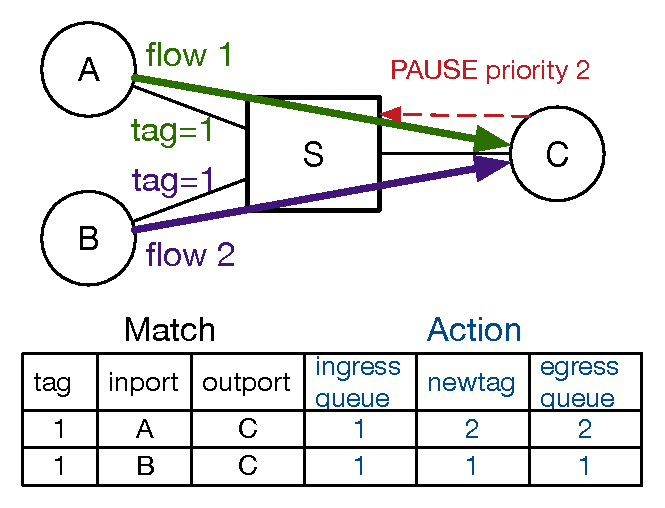
\includegraphics[width=0.43\textwidth] {figs/taggerdemon}
%	}
%	
%	\caption{Demonstration of \sysname{} implementation.}\label{fig:tagger_demon}
%\end{figure}
%
%
% \textbf{\sysname{} demonstration.} 


%\subsection{Lossless Priority Transition}\label{subsec:change_priority}
%
%
%Current PFC mechanism cannot prevent packet loss in some cases when packets change their priority classes along the path. An example can be found in Fig.~\ref{fig:queuetransition}.  \textcolor{red}{More description about this example will be added later.}
%
%As shown in Fig.~\ref{fig:queuetransition}(c), if we want a switch to pause its upstream device correctly, for packets of the same flow, the egress queue at last hop and the ingress queue at current hop must be of the same priority class. This means that we need to decouple ingress priority from egress priority in our implementation. 
%
%Then how to do this? We notice that Broadcom chipset based commodity switches, such as Arista 7060 switch, have alternative variables that can be used to decide the priority class of a packet inside the buffer management module. In normal case, only 1 variable will be used, and ingress priority is always the same as egress priority.
%
%We configure the switch to use different variables, denoted as ING$\_$PRIO and EG$\_$PRIO, to decide ingress priority and egress priority separately.   To set correct value for both NG$\_$PRIO and EG$\_$PRIO, we install some ACL rules at the ingress pipeline to  associate ING$\_$PRIO and EG$\_$PRIO  with (port, tag) information. These rules establish separate mappings from (port, tag) to ingress priority and egress priority, respectively.
%

%To ensure packets enter the correct lossless space at each hop, our solution requires the switch to classify packets into different priority classes based on  (port, tag) information. This can be done by installing some ACL rules at the ingress pipeline. As shown in Fig.~\ref{fig:switchmodel}, these rules will match the port $\#$ and value of tag, and assign packets to different priority calsses accordingly.
%
%To optimize the number of priorities needed for Clos and BCube topologies, we need to support flexible manipulation of tag value.  This can be done by installing some ACL rules at the egress pipeline. As shown in Fig.~\ref{fig:switchmodel}, these rules will calculate a new tag value for any outgoing packet based on the port $\#$ and old tag value, so the vaue of tag can be updated at each hop.

%\item \textbf{Egress pipeline}: The module to execute packet processing tasks after a packet leaves switch buffer. This module also has multiple match-action stages to do tasks such as egress ACL processing, packet tunneling and packet mirroring. Our (tag, port)-to-newtag mapping function is implemented as one match-action stage here.

%	Assuming the switch has n ports and supports k priority classes. Each port has k corresponding ingress queues and k corresponding egress queues to buffer packets of k priority classes. It is easy to know m = n*k. In the module, there is also a scheduler to forward packets to egress queues based on the packet metadata calculated at ingress pipeline.

%As shown in Fig.~\ref{fig:switchmodel}(b), the function of our modified PFC mechanism consists of four parts. 

%The PFC engine will track the instant queue lengths of all the VIQs (function (1)). If the queue length of some queue  $q_{in}^{i,j}$ exceeds the configured PFC threshold, PFC engine will generate a PAUSE message to pause the packet transmission of the immediate upstream node on priority class $j$-$1$ over the link connected with port $i$. If the queue length of $q_{in}^{i,j}$ becomes less than the threshold later, PFC engine will generate a RESUME message to resume the packet transmission over the previously paused link on priority class $j$-$1$ (function (2)).

%If some output port, say output port $i$, receives a PAUSE or RESUME message on priority class $j$ from its immediate downstream node, the PFC engine will then pause or resume the corresponding egress queue $q_{out}^{i,j}$, accordingly (function (3) and function (4)).

%The main difference between our modified PFC mechanism and the typical PFC mechanism is that, if the queue length of some queue $q_{in}^{i,j}$ at some network node exceeds the PFC threshold, PFC engine will pause the packet transmission of the immediate upstream node on priority class $j$-$1$ over the incoming link instead of on priority class $j$. This feature is important for realizing our TTL-based buffer management scheme, as we will introduce in the next.


%As shown in Fig.~\ref{fig:switchmodel}, the switch consists of five elements: switch port, forwarding engine, PFC engine, crossbar and switch buffer. The function of these elements are list as follows.
%
%%Fig.~\ref{fig:switchmodel}(a) shows the architecture of the switch model, which consists of a switching fabric and N line cards. Line cards are mainly used to receive/send packets and make routing/forwarding decisions. Switching fabric is a module to transfer packet cells from the input line card to the output line card. 
%
%\begin{itemize}
%	\item \textbf{Switch port}: The element to receive and send packets. Each switch port consists of an input port and an output port, and is connected with a link.
%	
%	\item \textbf{Forwarding engine}: The element to make the routing and/or switching decisions. In the forwarding engine, there is a module to decide the priority class of a packet based on the TTL value. 
%	
%	\item \textbf{PFC engine}: The element to perform PFC function.
%	
%	\item \textbf{Crossbar}: The element to switch packet cells from the ingress buffer to the egress buffer. 
%	
%	\item \textbf{Switch buffer}: The element to buffer incoming packets. We assume shared buffer in our model. In the ingress buffer, we use  virtual ingress queue (VIQ) to track the incoming packets. In the egress buffer, we use virtual egress queue (VEQ) to track the outgoing packets. Each VIQ is uniquely corresponding to an input port, while each VEQ is uniquely corresponding to an output port. As shown in Fig.~\ref{fig:switchmodel}, both VIQ and VEQ consist of k queues, with each queue corresponding to a priority class. A packet of priority class $j$ will enter the $j$-$th$ queue of its destined VIQ and VEQ.
%	
%	%    Note that in our switch model, when a packet in some VIQ is forwarded to some VEQ, this VIQ will not perform dequeue operation. Dequeue operation will be performed only after this packet leaves the switch buffer. This is because the purpose of using VIQ is to track the bytes of currently buffered packets received by an input port, such that PFC can work properly.
%	
%	\textbf{Discussion}: It is not always the case for switch to have both ingress buffer and egress buffer at the same time. It depends on the buffering strategy. If we adopt output-queued strategy, there will be no ingress buffer, and VIQs are simply some counters to record the bytes of buffered packets received by different input ports. If we adopt input-queued strategy~\cite{islip}, there will be no egress buffer, and VEQs can be simulated using virtual output	queuing technique~\cite{tinytera} at the ingress buffer. If we adopt the combined-input-and-output-queued strategy~\cite{chuang1999matching}, the switch will have both ingress buffer and egress buffer. The switching function of crossbar can also be virtual, not necessary to involve packet copying.
%	
%\end{itemize}
%
%\textbf{Enqueue and dequeue operations of VIQ and EIQ}: We use $q_{in}^{i}$ to denote VIQ $i$, and $q_{out}^{i}$ to denote VEQ $i$.
%Let $q_{in}^{i,j}$ be the $j$-$th$ queue of VIQ $i$, and $q_{out}^{i,j}$ be the $j$-$th$ queue of VEQ $i$ ($1\leq i \leq n$, $1 \leq j \leq k$). The dequeue and enqueue operatons of VIQ and VEQ are performed as follows:
%
%\begin{enumerate}
%	\item  Packet $p$ of priority class $j$ enters the switch buffer via input port $i_1$: VIQ $i_1$ performs enqueue operation and puts packet $p$ to the tail of $q_{in}^{i_1,j}$.
%	
%	\item  Packet $p$ in the head of $q_{in}^{i_1,j}$ is forwarded to VEQ $i_2$:  VEQ $i_2$ performs enqueue operation and puts packet $p$ to the tail of $q_{out}^{i_2,j}$. At the same time, head point of $q_{in}^{i_1,j}$ is moved to the next packet currently queued in $q_{in}^{i_1,j}$. Note that dequeue operation of packet $p$ will not be performed at $q_{in}^{i_1,j}$ at this point in time. 
%	
%	\item  Packet $p$ in the head of $q_{out}^{i_2,j}$ is forwarded to output port $i_2$: VEQ $i_2$ performs dequeue operation and removes packet $p$ from $q_{out}^{i_2,j}$.  VIQ $i_1$ performs dequeue operation and removes packet $p$ from $q_{in}^{i_1,j}$ (say packet $p$ was previously forwarded from $q_{in}^{i_1,j}$ to $q_{out}^{i_2,j}$). 
%\end{enumerate}
%
%Note that, dequeue operation is performed at corresponding VIQ only after packet $p$ leaves the switch buffer. This is because the purpose of using VIQ is to track the bytes of currently buffered packets received by an input port, such that PFC can work properly.



